\documentclass{beamer}
% Author: Alick Zhao <alick9188@gmail.com>
% Author: Zamir Sun <zsun@fedoraproject.org>

% This file is modified from a solution template for:

% - Giving a talk on some subject.
% - The talk is between 15min and 45min long.
% - Style is ornate.

% Copyright 2004 by Till Tantau <tantau@users.sourceforge.net>.
%
% In principle, this file can be redistributed and/or modified under
% the terms of the GNU Public License, version 2.
%
% However, this file is supposed to be a template to be modified
% for your own needs. For this reason, if you use this file as a
% template and not specifically distribute it as part of a another
% package/program, I grant the extra permission to freely copy and
% modify this file as you see fit and even to delete this copyright
% notice.

\mode<presentation>
{
  \usetheme{Madrid}
  \setbeamercovered{transparent}
\definecolor{fedorablue}{RGB}{60,110,180}
\definecolor{fedoradarkblue}{RGB}{41,65,114}
\definecolor{fedoradarkgrey}{RGB}{76,76,76}
\setbeamercolor*{palette primary}{fg=white,bg=fedorablue}
\setbeamercolor*{palette secondary}{fg=white,bg=fedoradarkblue}
\setbeamercolor*{palette tertiary}{fg=white,bg=fedorablue}
\setbeamercolor*{palette quaternary}{fg=white,bg=black}
}

\usepackage{graphicx}
\graphicspath{{fig/}}
\usepackage{listings}
\usepackage{xspace}
\usepackage{fontspec}
\usepackage[CJKchecksingle]{xeCJK}

\usepackage{hyperxmp}
\hypersetup{
pdfauthor={Alick Zhao, Zamir Sun},
pdfcopyright={Copyright (C) 2014 by Alick Zhao and Zamir Sun.
Licensed under CC-BY-SA 4.0. Some rights reserved.
This work is based on Matthew Miller's previous work.
You need to follow the logo usage guideline to use the Fedora logo.},
pdflicenseurl={http://creativecommons.org/licenses/by-sa/4.0/},
}

% xeCJK conf setup
\punctstyle{kaiming}

\setCJKmainfont[BoldFont={WenQuanYi Micro Hei},
ItalicFont={AR PL UKai CN}]{AR PL UMing CN}
\setCJKsansfont{WenQuanYi Micro Hei}
\setCJKmonofont{WenQuanYi Micro Hei Mono}

\setCJKfamilyfont{zhsong}{AR PL UMing CN}
\setCJKfamilyfont{zhhei}{WenQuanYi Zen Hei}
\setCJKfamilyfont{zhkai}{AR PL UKai CN}

\newcommand*{\songti}{\CJKfamily{zhsong}} % 宋体
\newcommand*{\heiti}{\CJKfamily{zhhei}}   % 黑体
\newcommand*{\kaishu}{\CJKfamily{zhkai}}  % 楷书

\title{What's New in Fedora?}

\author[alick \& zsun] % (optional, use only with lots of authors)
{Alick Zhao and Zamir SUN\\ \texttt{\{alick,zsun\}@fedoraproject.org}}

\date[Fedora 21 Release Party] % (optional)
{Jan 24, 2015}

\subject{Fedora, Fedora.next}

% Delete this, if you do not want the table of contents to pop up at
% the beginning of each subsection:
\AtBeginSection[]
{
  \begin{frame}<beamer>{Outline}
    \tableofcontents[currentsection]
  \end{frame}
}

% If you wish to uncover everything in a step-wise fashion, uncomment
% the following command:

%\beamerdefaultoverlayspecification{<+->}

\hypersetup{
%pdfpagemode=FullScreen,
breaklinks=false,
}

\logo{
\includegraphics[height=.15\textheight]{fedora_logo_cmyk.pdf}}

\begin{document}

\begin{frame}
  \titlepage
\end{frame}

\begin{frame}{Outline}
  \tableofcontents
  % You might wish to add the option [pausesections]
\end{frame}


% Since this a solution template for a generic talk, very little can
% be said about how it should be structured. However, the talk length
% of between 15min and 45min and the theme suggest that you stick to
% the following rules:

% - Exactly two or three sections (other than the summary).
% - At *most* three subsections per section.
% - Talk about 30s to 2min per frame. So there should be between about
%   15 and 30 frames, all told.

\section{Introduction}

\begin{frame}{About Me}
  \begin{itemize}
    \item Zamir SUN, aka zsun
    \item Linux user
    \item Fedora contributor
    \item Email: \texttt{zsun@fedoraproject.org}
  \end{itemize}
\end{frame}

%\begin{frame}{About Me}
%  \begin{columns}
%    \begin{column}{.75\textwidth}
%  \begin{itemize}
%    \item Master student
%    \item Linux hobbyist
%    \item Fedora contributor
%    \item TUNA member
%    \item ID: alick, alick9188
%    \item Email: \texttt{alick@fedoraproject.org}
%  \end{itemize}
%    \end{column}
%    \begin{column}{.25\textwidth}
%      \begin{figure}[htbp]
%        \centering
%        
\includegraphics[width=.6\textwidth]{wu.jpg}
%      \end{figure}
%    \end{column}
%  \end{columns}
%\end{frame}

\begin{frame}{Fedora in a Nutshell}
  \begin{columns}
    \begin{column}{.5\textwidth}
  \begin{itemize}
    \item GNU/Linux distro
      \begin{itemize}
        \item Community driven
        \item Sponsored by Red Hat
        \item Upstream to RHEL, CentOS
      \end{itemize}
    \item 20 releases in 10 years
    \item Fedora 21 as the first release of Fedora.Next
  \end{itemize}
    \end{column}
    \begin{column}{.5\textwidth}
      \begin{figure}[htbp]
        \centering
        
\includegraphics[width=.6\textwidth]{tenyears.jpeg}
      \end{figure}
    \end{column}
  \end{columns}
\end{frame}

\begin{frame}{Fedora Four Foundations}
  \begin{figure}[htbp]
    \centering
    
\includegraphics[height=.7\textheight]{four_foundations.pdf}
  \end{figure}
\end{frame}

\begin{frame}{Inside Fedora}
  \begin{itemize}
    \item Sub-projects
      \begin{figure}[htbp]
        \centering
        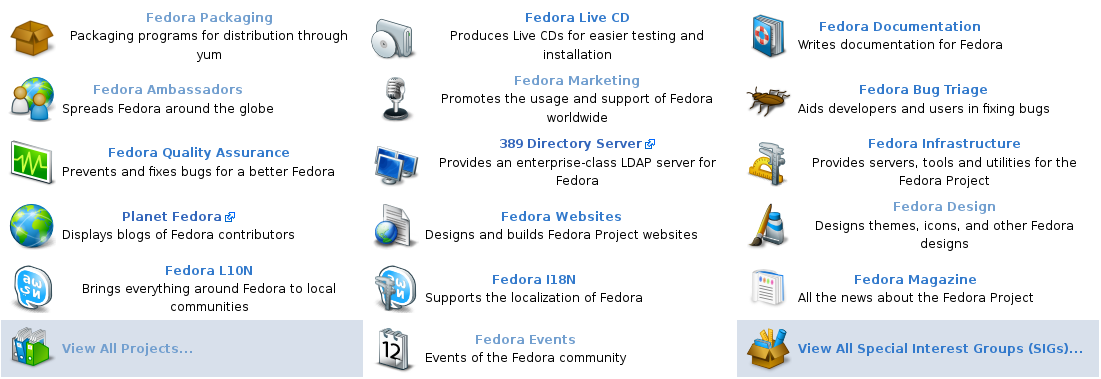
\includegraphics[width=.9\textwidth]{subprojects.png}
      \end{figure}
  \end{itemize}
\end{frame}

\section{Fedora.next Proposal}
\begin{frame}
  \frametitle{Why Fedora.next?}
  \begin{itemize}
    \item The world is changing:
      \begin{itemize}
        \item Cloud! OpenStack! OpenShift!
        \item Containers! Docker! CoreOS!
        \item GitHub, Rubygem, NPM
        \item Base OS considered boring
        \item Not just us: Debian, Ubuntu, openSUSE all \alert{no
          longer cool}
      \end{itemize}
  \end{itemize}
  \begin{beamercolorbox}[center,ht=2ex,dp=0.5ex,rounded=true]{block body}
    {\centering ``Is distribution-level package management
    obsolete?''}
  \end{beamercolorbox}
\end{frame}

\begin{frame}{Fedora's Mission}
  \begin{beamercolorbox}[center,ht=4ex,dp=0.5ex,rounded=true]{block body}
    {\centering The Fedora Project's mission is to lead the advancement of free and
  open source software and content as a collaborative community.}
  \end{beamercolorbox}
\end{frame}

\begin{frame}{Fedora.next}
  \begin{itemize}
    \item Additive
    \item Incremental improvement
    \item Planning, direction-setting
  \end{itemize}
\end{frame}

\begin{frame}{Fedora Rings Model}
  \begin{columns}
    \begin{column}{.5\textwidth}
  \begin{itemize}
    \item Ring 0: Minimal Core
    \item Ring 1: Common Base Platform
    \item Ring 2: Environments \& Stacks
    \item Ring 3: Applications
  \end{itemize}
    \end{column}
    \begin{column}{.5\textwidth}
      \begin{figure}[htbp]
        \centering
        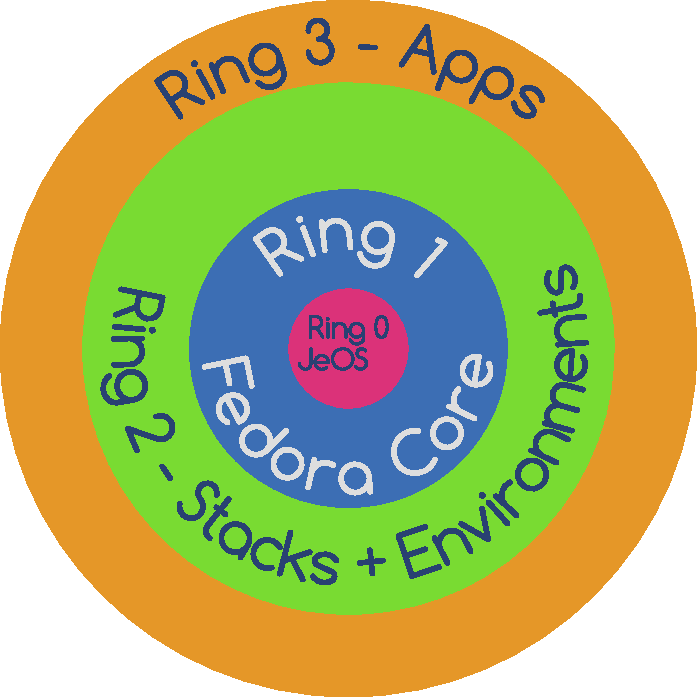
\includegraphics[width=.8\textwidth]{fedora-next-ring.pdf}
      \end{figure}
    \end{column}
  \end{columns}
\end{frame}

%\begin{frame}{Fedora Products Proposal}
%  \begin{itemize}
%    \item Fedora Workstation
%    \item Fedora Server
%    \item Fedora Cloud
%  \end{itemize}
%\end{frame}

\section{What's new in Fedora 21}
% notable features available in Fedora 21
\begin{frame}{Products}
  \begin{itemize}
    \item Fedora Workstation
      \begin{itemize}
        \item GNOME 3.14
        \item GNOME Wayland sessions
      \end{itemize}
    \item Fedora Server
      \begin{itemize}
        \item Rolekit, role management
        \item Cockpit, system management
      \end{itemize}
    \item Fedora Cloud
      \begin{itemize}
        \item EC2 images
        \item Docker images
        \item Atomic images
      \end{itemize}
  \end{itemize}
\end{frame}

\begin{frame}{Beyond}
  \begin{itemize}
    \item Non products
      \begin{itemize}
        \item Spins: KDE, ARM, \ldots
      \end{itemize}
    \item Websites
      \begin{itemize}
        \item getfedora.org
        \item Fit for mobile devices
      \end{itemize}
  \end{itemize}
\end{frame}

% need to check the status
\begin{frame}{Fedora 21}
  \begin{itemize}
    \item Software collections
    %\item Fedora Playground: COPR
    \item Wayland for GNOME, GDM still run on X
    \item Big data: Apache HBase/Hive/Pig/Spark \ldots
    \item \url{https://fedoraproject.org/wiki/Releases/21/ChangeSet}
  \end{itemize}
\end{frame}


\section{Ongoing Work}

\begin{frame}{Governance}
  \begin{itemize}
    \item Working groups:
      \begin{itemize}
        \item One each for the products
        \item One for Base Design
        \item One for Environments \& Stacks
      \end{itemize}
    \item Each working group: a group of voting members
    \item FESCo, Design, QA, etc still there
    \item FOSCo, replacement and extend of FAmSCo
  \end{itemize}
\end{frame}

\begin{frame}{You Can Contribute!}
  \begin{itemize}
    \item Spread the message
    \item Join the discussion
      \begin{itemize}
        \item Mailing list
        \item IRC
      \end{itemize}
    \item Design, Code, Document, Translate, etc.
    \item Fedora Join SIG
  \end{itemize}
\end{frame}

\begin{frame}{Where are we?}
  \begin{figure}[htbp]
    \centering
    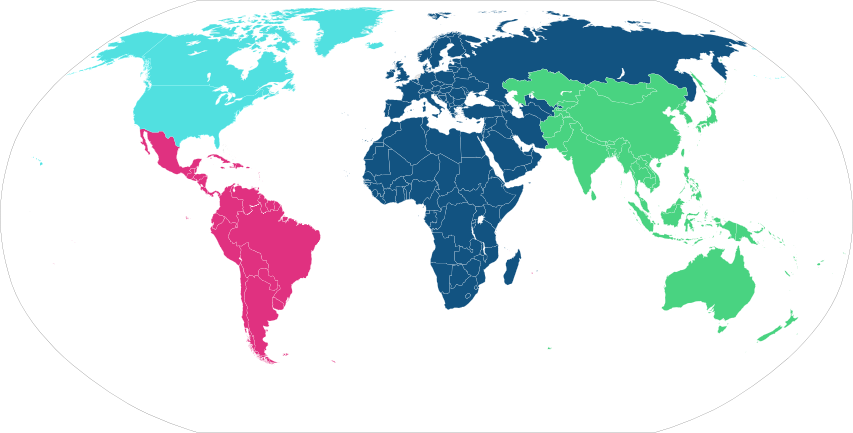
\includegraphics[width=\textwidth]{Ambassador-World-Map.png}
  \end{figure}
\end{frame}

\section*{Summary}

\begin{frame}{Summary}
  % Keep the summary *very short*.
  \begin{itemize}
  \item Fedora: Freedom, Friends, Features, First
  \item Fedora.next: More Agile
  \item Join Fedora: Meet the community
  \end{itemize}
\end{frame}

\section*{Appendix}

\begin{frame}{Appendix}
  \begin{itemize}
    \item This slides: \url{https://github.com/alick9188/f21relparty}
    \item Matthew Miller's slides: \url{http://mattdm.org/fedora/next2014/}
  \end{itemize}
\end{frame}

\begin{frame}
  \begin{center}
    {\LARGE Thanks!
    \bigskip

    Questions?}

  \end{center}
\end{frame}

\end{document}
%%% vim: set sw=2 isk+=\: et tw=70 formatoptions+=mM:
